\documentclass[11pt,a4paper]{article}
\usepackage{tikz}
\usetikzlibrary{arrows, arrows.meta}
\usepackage[utf8]{inputenc}
\usepackage{amsfonts}
\usepackage{float}
\usepackage{graphicx}
\usepackage[normalem]{ulem}
\usepackage{setspace}
\usepackage[document]{ragged2e}
\usepackage{fancyhdr}
\usepackage[backend=biber, style=apa, citestyle=authoryear, autocite=inline]{biblatex}
\DeclareLanguageMapping{english}{english-apa}
\addbibresource{cf_refs.bib}
\renewcommand*{\nameyeardelim}{\addcomma\space}
\usepackage[left=2.5cm,right=2.5cm,top=2.5cm,bottom=2.5cm]{geometry}
\usepackage{gb4e}
\author{Semih Can Aktepe}
\title{An Essay on Turkish Syntax}

\spacing{1.25}

\pagestyle{fancy}
\fancyhf{}
\lhead{Semih Can Aktepe}
\rhead{COGS532}
\cfoot{\thepage}

\begin{document}\thispagestyle{empty}
\maketitle
\justify
\section{What is different in Turkish?}
Turkish is an agglutinating language that takes its verbs to the final position of its sentences. When the structures are formed in Turkish, the derivational and inflectional morphemes are added to the end of the stems. Therefore, although the syntactic operations can be partly explained by the morphological theory in Turkish, the issues in this essay are discussed regarding the syntactic theory. The basic canonical word order of Turkish is Subject-Object-Verb (SOV), but there is no fixed word order. Thus, Turkish has a scrambling word order, meaning that SVO, OSV, OVS, VSO and VOS word orders are possible on the surface as well. These permutations may sometimes lead to ambiguity, yet highly inflectional morphology of Turkish relative to that of English allows the listeners and readers not to confuse among different word orders as in (1a) and (1b).
\begin{exe}
		\ex
			\begin{xlist}
				\ex Ahmet kedileri besledi.\\
				Ahmet-NOM cats-ACC feed-PAST\\
				``Ahmet fed the cats."
				\ex Kedileri besledi Ahmet.\\
				cats-ACC feed-PAST Ahmet-NOM\\
				``Ahmet fed the cats."
			\end{xlist}
	\end{exe}
The scrambling word order of Turkish does not mean that the words can be moved anywhere in the sentence without any restriction. Not every head can be nested anywhere at random. For instance, the nouns in the sentences in (1) are case-marked\footnote{The term \emph{case-marked} refers to the fact that the noun bears a case.}, and all six word orders are grammatical and acceptable. Nevertheless, when the nouns are not case-marked, their positioning is restricted as in (2).
\begin{exe}
		\ex
			\begin{xlist}
				\ex Ahmet kedi besliyor.\\
				Ahmet-NOM cat feed-PRES\\
				``Ahmet feeds a cat."
				\ex *Kedi Ahmet besliyor.\\
				*cat Ahmet-NOM feed-PRES
			\end{xlist}
	\end{exe}
The same restriction is also valid for the adjuncts such as adverbial, adjectival and prepositional phrases.
\begin{exe}
		\ex
			\begin{xlist}
				\ex Merve hızlı koşar.\\
				Merve-NOM fast run-AOR\\
				``Merve runs fast."
				\ex *Hızlı Merve koşar.\\
				*fast Merve-NOM run-AOR
				\ex Hızlı koşar Merve.\\
				fast run-AOR Merve-NOM
			\end{xlist}
	\end{exe}
In the example (3b), unless the word \emph{hızlı} is taken as an adjective, the sentence (3b) is ungrammatical. Likewise, in the situation that \emph{hızlı} is regarded as an adjective, the sentences in (3a) and (3c) are also ungrammatical.
\subsection{Agreement}
In Turkish, the subject and the verb agree with each other through some inflectional person and number markings. One exception is that 3rd person plural suffix can sometimes be omitted, making it ambiguous with the 3rd person singular. Other than that, each person has a unique suffix. That’s why, even if the subject is dropped\footnote{Parameters will be discussed in the following parts.}, the person and number information can be gathered from the inflection of the verb. When the subject is omitted, it is replaced by a phonologically absent syntactic particle \emph{pro}\footnote{This is \textbf{little} pro, there is also \textbf{big} PRO which is used to replace the subjects in control sentences.}.
\begin{exe}
		\ex
			\begin{xlist}
				\ex \emph{pro} bu akşam geleceğim.\\
				this evening come-FUT-1pSin\\
				``I will come this evening.”
				\ex \emph{pro} bu akşam geleceğiz.\\
				this evening come-FUT-1pPlu\\
				``We will come this evening.”
			\end{xlist}
	\end{exe}
Besides subject-verb agreement, possessor and possessed items also agree with each other again through some overt markings.
\begin{exe}
		\ex
			\begin{xlist}
				\ex Sizin arabanız\\
				You (all)-GEN car-POSS\\
				``Your car"
				\ex Onların arabası\footnote{In this example, \emph{arabası} also agrees with 3rd person singular possessor \emph{onun}, which is an instance of ambiguity in Turkish.}\\
They-GEN car-POSS\\
``Their car"
			\end{xlist}
	\end{exe}
In short, the agreement between the structures in Turkish is motivated by case-marking and morphological operations in general.\footnote{You can refer to \textcite{oflazer} for further information about Turkish morphology and check the following website for the morphological modelling of Turkish verbs. \url{https://github.com/tschomski/modelling-of-turkish-verbs}}
After all, Turkish morphology sometimes does not reveal the agreement between subjects and verbs, which causes structural ambiguity in some structures such as (6).
\begin{exe}
\ex 
\gll Ayşe sınavı geçtiği için çok mutlu.\\
Ayşe-NOM exam-ACC pass for very happy.\\
\glt Ayşe_{i} [\emph{pro}/o_{j} sınavı geçtiği için] çok mutlu.\\
Ayşe_{i} is very happy that she_{i/j} has passed the exam.
\end{exe}
The sentence in (6) suggests two different meanings: first is that Ayşe passes the exam and she is happy with the result; second is that someone else passes the exam and Ayşe is happy with that. The similar phenomenon can be observed in the binding principles proposed by \textcite{government}. The Principle A of the Binding Theory states that a reflexive must be bound by a local c-commanding antecedent as in (7).
\begin{exe}
\ex Emre_{i} [Cem'in_{j} \textbf{kendini}_{j/*i/*k}] suçladığını anladı.\\
Emre Cem-GEN kendi-ACC blame understood\\
``Emre_{i} realized that Cem_{j} is blaming himself_{j/*i/*k}." 
\end{exe}
Furthermore, the Principle B of the Binding Theory posits that a pronoun must be free  within its governing category; i.e. not bound by anything in its local clause as in (8).
\begin{exe}
\ex Yeliz_{i} [Tuğba'nın_{j} \textbf{onu}_{i/k/*j} affettiğini] fark etti.\\
Yeliz Tuğba-GEN him/her-ACC forgive noticed\\
``Yeliz_{i} noticed that Tuğba_{j} forgave him/her_{i/k/*j}."
\end{exe}
\textcite{martinaanap} show that Turkish native speakers find sentences like (7) acceptable even when the anaphora refer to their long distance antecedent but do not accept when they are bound to an extra-sentential antecedent, which is surprising considering the violation of the Principle A of the Binding Theory. As for the sentences like (8), people do not find them acceptable when the pronouns refer to a local antecedent, which still adheres to the Principle B of the Binding Theory. The more interesting finding is that when people are given a context, they tend to find all kinds of binding relations relatively more acceptable than when there is no context bias\footnote{See \textcite{martinaanap} for full results.}. Therefore, unlike English which strictly conforms to the syntactic rules, Turkish does not stick to some syntactic rules, rather keeping pragmatic constraints over syntactic ones in some particular cases.
\subsection{Parameters}
\textcite{minimalist} suggests that natural language syntax is described according to general rules that are universal, and a set of optional variants that vary among languages. This framework is called \emph{Principles and Parameters}. As mentioned above, the subjects can be dropped in Turkish, so Turkish is called a \emph{pro-drop} language. When we further compare English and Turkish, as known, the verbs assign theta roles to their arguments. For example, the transitive verb \emph{see} assigns its subject \emph{the one who sees} \textsc{Experiencer} theta-role, and \textsc{Theme} theta-role to its object\footnote{These do not necessarily have to be subjects or objects, they can sometimes become propositions based on the verb's theta grid.} \emph{the seen}. These assignments happen overtly in English. Hence, when the assigner verb has more or less argument than it can assign theta-role to, the sentence becomes ungrammatical. However, this does not hold in Turkish since the complements can also be dropped in Turkish, for it is a \emph{complement-drop} language. See the examples in (9).
\begin{exe}
		\ex
			\begin{xlist}
				\ex A: Duş aldın mı?\\
				B: Evet, aldım.
				\ex A: Did you take a shower?\\
				B: *Yes, I took.
			\end{xlist}
	\end{exe}
As the examples in (9) imply, Turkish does not need any overt markee, whereas English does. The only way to make the English example grammatical is to substitute the whole predicate \emph{took a shower} with \emph{did}. In this case, \emph{Yes, I did} makes the sentence grammatical. Having said that \emph{Pro-Drop Parameter} and \emph{Complement-Drop Parameter} are different in Turkish than in English, there is one more parameter to speak of. At the very beginning, it is said that Turkish takes its verbs to the end of the sentences. Therefore, another parameter that differentiates Turkish from English is the \emph{Head Directionality Parameter}. When the phrases in English are investigated, their heads are always on left side of the tree, thus making it a head-initial language. However, in Turkish, it is vice versa. Hence, Turkish is a \emph{head-final} language. Compare the prepositional phrase in English and post-positional phrase in Turkish given below.\\
\begin{figure}[H]
\begin{center}
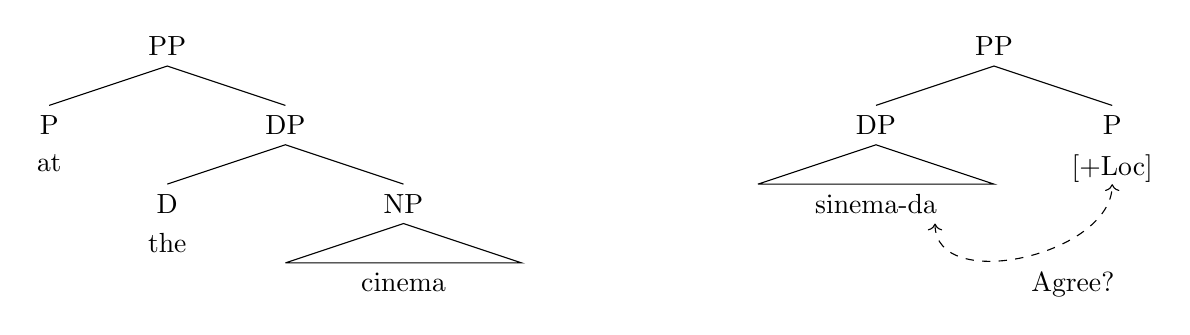
\begin{tikzpicture}
\draw (0,0) -- (1.5,0.50) -- (3,0);
\node at (1.5,0.75) {PP};
\node at (0,-0.25) {P};
\node [below] at (0,-0.5){at};
\draw (1.5,-1) -- (3,-0.5) -- (4.5,-1);
\node at (3,-0.25) {DP};
\node at (1.5,-1.25) {D};
\node [below] at (1.5,-1.5) {the};
\draw (3,-2) -- (4.5,-1.5) -- (6,-2) -- (3,-2);
\node at (4.5,-1.25) {NP};
\node [below] at (4.5,-2) {cinema};
\draw (10.5,0) -- (12,0.50) -- (13.5,0);
\node at (12,0.75) {PP};
\node at (13.5,-0.25) {P};
\node [below] at (13.5,-0.5) {[+Loc]};
\node at (10.5,-0.25) {DP};
\draw (9,-1) -- (10.5,-0.5) -- (12,-1) -- (9,-1);
\node [below] at (10.5,-1) {sinema-da};
\draw [dashed, <->] (11.25,-1.5) to [out=-90,in=-90] (13.5,-1);
\node [below] at (13,-2) {Agree?};
\end{tikzpicture}
\end{center}
\caption{The comparison of prepositional phrase in English (left) and post-positional phrase in Turkish (right) on syntax trees.}
\end{figure}
\section{How does Turkish work?}
Turkish does not have the movement operations such as V-to-T movement in French and Irish and wh-movement in English (See the example 10 and figure 2).
\begin{exe}
\ex
John'un ne yaptığını düşünüyorsun?
\gll [\emph{pro} [John'un_{DP} [ne_{WH} yaptığını_{V}]_{VP}]_{CP} düşünüyorsun_V?]_{CP}\\
\emph{(you)} John-GEN what do think-PRES-2pSin\\
\glt ``What do you think John has done?"
\end{exe}

\begin{figure}[H]
\begin{center}
\begin{tikzpicture}
\node [below] at (0,0) {What do you think \emph{t_{i}} John has done \emph{t_{i}}?};
\draw [dashed, ->] (3.05,-0.5) to [out=-90,in=-90] (0.15,-0.5);
\draw [dashed, ->] (0,-0.5) to [out=-90,in=-90] (-2.9,-0.5);
\end{tikzpicture}
\end{center}
\caption{The movement of WH-Phrase}
\end{figure}
\noindent In yes/no questions, while English has some operations such as \emph{do-support} and \emph{subject-auxiliary inversion}, the question clitic \emph{-mH} is placed at the end of the sentence in Turkish, occupying Spec-CP position of the matrix CP, and it is licensed by C-head where the question feature is checked (See example 11). 
\begin{exe}
\ex
\gll [[Şeyhmus_{DP} [basketbol_{DP} oynar_{V}]_{VP}]_{TP} mı_{Q}?]_{CP}\\
Şeyhmus-NOM basketball play-AOR-3pSin Q-clitic\\
\glt ``Does Şeyhmus play basketball?"
\end{exe}
As mentioned before, English  follows the phrase structure rules more strictly than Turkish since the scrambling word order apparently makes the application of these re-write rules relatively harder. However, when canonical word order of Turkish, which is SOV, is taken into account, Turkish seems to follow these rules anyway, yet the placement of some phrases such as the intervention of PP's or AdvP's between objects and verbs creates other problems. Similar problems can be noticed in English as in resumptive pronouns \emph{(John, \textbf{he} is a good guy.)}, which seemingly infringes the re-write rules. In this resumptive pronoun example, the matter is, rather than focusing on \emph{John's being a good guy}, that we focus on \emph{John} himself. Therefore, our \emph{topic} in the sentence is changed by the given information in the discourse. Speaking of a different point, information is not always delivered in the conversation. If the new information is not expressed in the discourse, then this information is called \emph{focus}. Without any special intonation and stress, focus is the VP in English. The focus shift to another phrase is shown in the example (12).
\begin{exe}
\ex A: To Whom did Mary give the book?\\
B: [To Mark]_{F}, Mary gave the book.
\end{exe}
In the example above, the listeners of the sentence can understand that the prepositional phrase can be traced back to its original position in the canonical word order. Therefore, they know the information structure of the sentence. Likewise, Turkish speakers know the information structure of their sentences. Thus, they can also shift the topic or focus of their sentences depending on whether the information has been provided for the interlocutor previously. \textcite{rizzi} introduces \emph{Topic Phrase} and \emph{Focus Phrase} which take place on the left edge of every clause. Consequently, considering what discourse effect the focused or topicalized phrase has, that phrase moves into the specifier position of Topic Phrase or Focus Phrase in scrambling languages\footnote{This is not necessarily peculiar to scrambling languages; such an approach is because the issue of this essay is Turkish language.} such as Turkish and Japanese. How this system works in Turkish is given below on the sentence \emph{Ahmet kedileri evde besliyor}.
\begin{figure}[H]
\begin{tikzpicture}
\draw (0,0) -- (1.5,0.5) -- (3,0);
\node at (1.5,0.75) {TopicP};
\node at (0,-0.25) {Ahmet};
\draw (1.5,-1) -- (3,-0.5) -- (4.5,-1);
\node at (3,-0.25) {Topic'};
\node at (1.5,-1.25) {TopicP};
\node at (4.5,-1.25) {Topic};
\draw (0,-2) -- (1.5,-1.5) -- (3,-2);
\node at (0,-2.25) {kedileri};
\node at (3,-2.25) {Topic'};
\draw (1.5,-3) -- (3,-2.5) -- (4.5,-3);
\node at (1.5,-3.25) {TP};
\node at (4.5,-3.25) {Topic};
\draw (0,-4) -- (1.5,-3.5) -- (3,-4);
\node at (0,-4.25) {DP};
\node [below] at (0,-4.5) {Ahmet};
\node [blue, below] at (0,-5){[$\phi$ $3,sg$]};
\node at (3,-4.25) {T'};
\draw (1.5,-5) -- (3,-4.5) -- (4.5,-5);
\node at (1.5,-5.25) {VP};
\node at (4.5,-5.25) {T};
\node [blue, below] at (4.5,-5.35){[FIN +]};
\node [blue, below] at (4.5,-5.75){[$\phi$^{(u)} $\checkmark$]};
\draw (0,-6) -- (1.5,-5.5) -- (3,-6);
\node at (0,-6.25) {$\langle$DP$\rangle$};
\node [below]at (0,-6.5) {\sout{Ahmet}};
\node [blue, below] at (0,-7){[FIN^{(u)} $\checkmark$]};
\node at (3,-6.25) {V'};
\draw (1.5,-7) -- (3,-6.5) -- (4.5,-7);
\node at (1.5,-7.25) {PP};
\node [below] at (1.5,-7.5) {evde}; 
\node at (4.5,-7.25) {V'};
\draw (3,-8) -- (4.5,-7.5) -- (6,-8);
\node at (3,-8.25) {DP};
\node [below] at (3,-8.5) {kedileri};
\node [blue, below] at (3,-9){[CAT^{(u)} $\checkmark$]};
\node at (6,-8.25) {V};
\node [below] at (6,-8.5) {besliyor};
\node [blue, below] at (6,-9) {[CAT v]};
\draw [red, ->] (0,-7) to [out=240,in=180] (-0.65,-5);
\draw [->] (-0.75,-4.75) to [out=150,in=180] (-0.7,-0.25);
\draw [->] (2.5,-9) to [out=240,in=180] (-0.75,-2.25);
\draw [magenta, dashed, <->] (3,-9.75) to [out=-90,in=-90] (6,-9.75);
\draw [magenta, dashed, <->] (0.25,-7.65) to [out=-90,in=90] (4,-5.5);
\draw [magenta, dashed, <->] (0.75,-5) to [out=90,in=30] (5.25,-6.15);
\end{tikzpicture}
\caption[Caption for LOF]{The syntax tree representation of the sentence\footnotemark}
\end{figure}
\footnotetext{The red arrow indicates subject head movement, magenta dashed arrows introduce feature checking and the other black arrows show topic movement.}
\noindent The question raised here might be \emph{what about the post-verbal phrases in such sentences as \textbf{Besliyor Ahmet evde kedileri}?} The possible answer is to switch specifier of the TopicP's and FocusP's to the right periphery rather than just limiting the proposal of \textcite{rizzi} to the left periphery, yet what issues this extension raises is the topic of further analysis.
\printbibliography
\end{document}